% !TeX root = ../main.tex
\chapter{Overview}\label{chapter:overview}

\section{System Overview}
The logging system is a critical component of the GDPRuler project, designed to maintain comprehensive audit trails of all operations performed on personal data within the underlying key-value store. These logs are tamper-evident, encrypted for security, compressed for efficient storage and structured for retrieval that does not interfere with ongoing logging. The system operates as an append-only logging mechanism, providing high throughput for write operations while supporting occasional bulk export for compliance reporting or auditing.

\section{Design Goals}
The logging system's architecture is built upon several fundamental design goals that directly address the requirements of secure GDPR compliance logging:

\begin{enumerate}
    \item \textbf{Performance Optimization}: The system prioritizes high write throughput, recognizing that logging operations must not become a bottleneck in the broader GDPRuler framework. This is achieved through a batched writing approach and efficient queue-based architecture.
    \item \textbf{Scalability}: The architecture supports concurrent operations through a queue-based design and multiple writer threads, allowing the system to handle high-volume logging requirements efficiently.
    \item \textbf{Data Integrity and Security}: The system implements tamper-evidence through cryptographic chaining, ensuring that any unauthorized modifications to the logs can be detected. This is complemented by encryption to protect the sensitive log contents.
    \item \textbf{Operational Flexibility}: The system supports occasional log exports and archival operations without impacting ongoing logging activities, facilitating compliance audits and long-term data retention requirements.
\end{enumerate}

\begin{figure}
    \centering
    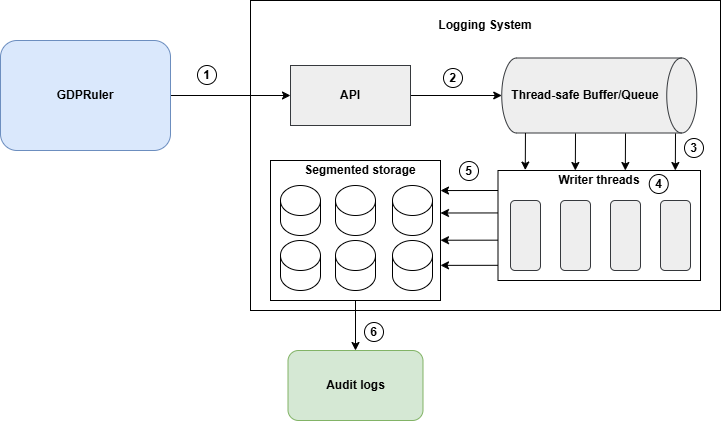
\includegraphics[scale=0.4]{images/systemfigure.png}
    \caption{GDPRlogger system figure}
    \label{fig:systemfigure}
\end{figure}

\section{System Workflow}
The logging process follows a streamlined workflow designed to maximize efficiency and reliability:
\begin{enumerate}
    \item \textbf{Log Entry Creation}: When the GDPRuler engine processes a personal data related operation, it generates a log entry containing relevant metadata such as timestamps, action types, and data locations.
    \item \textbf{Enqueuing}: Log entries are immediately enqueued through the logging API, allowing the calling process to continue without waiting for disk operations.
    \item \textbf{Batch Processing}: Dedicated writer threads continuously monitor the queue, collecting entries into batches for optimized processing.
    \item \textbf{Security Processing}: Batched entries undergo security treatments including compression and encryption, with cryptographic chaining applied to ensure tamper-evidence.
    \item \textbf{Persistent Storage}: Processed batches are written to append-only segment files, with new segments created based on size or time thresholds.
    \item \textbf{Export and Verification}: When required, closed segments can be exported for auditing purposes, with the system performing decryption, decompression, and hash chain verification to ensure data integrity throughout the export process.
\end{enumerate}

\section{System Components}
The logging system consists of four primary components, each serving a specific function.The \textbf{logging API} provides the interface for log entry submission, handling the initial serialization of metadata and ensuring quick response times through asynchronous processing. The \textbf{buffer Queue} acts as the system's central coordination mechanism, implementing a thread-safe, lock-free design to manage the flow of log entries from submission to processing. \textbf{Writer threads} perform the core processing of log entries, managing compression, encryption, and cryptographic chaining while ensuring efficient disk operations through batched writing. The \textbf{segmented storage} manages the physical storage of log data, implementing an append-only design with segment-based organization to facilitate efficient exports and archives while maintaining data integrity.\\

\noindent
Each component is designed to operate independently while maintaining strict coordination through well-defined interfaces. By adhering to these principles and workflows, the logging system achieves the dual goals of high performance and robust GDPR compliance, ensuring that all logged transactions are secure and verifiable.